\chapter{Arquitetura do Projeto}

Para a execução dos testes de performance foi desenvolvido um Web service com as principais operações necessárias para manter os dados do AFD. O objetivo ao se escolher realizar os testes de performance via Web service foi o de flexibilizar ao máximo as implementações em diversos bancos de dados. O Web service foi desenvolvido utilizando-se a linguagem de programação python e, adicionalmente, foi utilizado o framework web2py. A diagramação da arquitetura pode ser vista na figura \ref{fig:arquitetura}

	\begin{figure}[!htbp]
		\begin{center}
			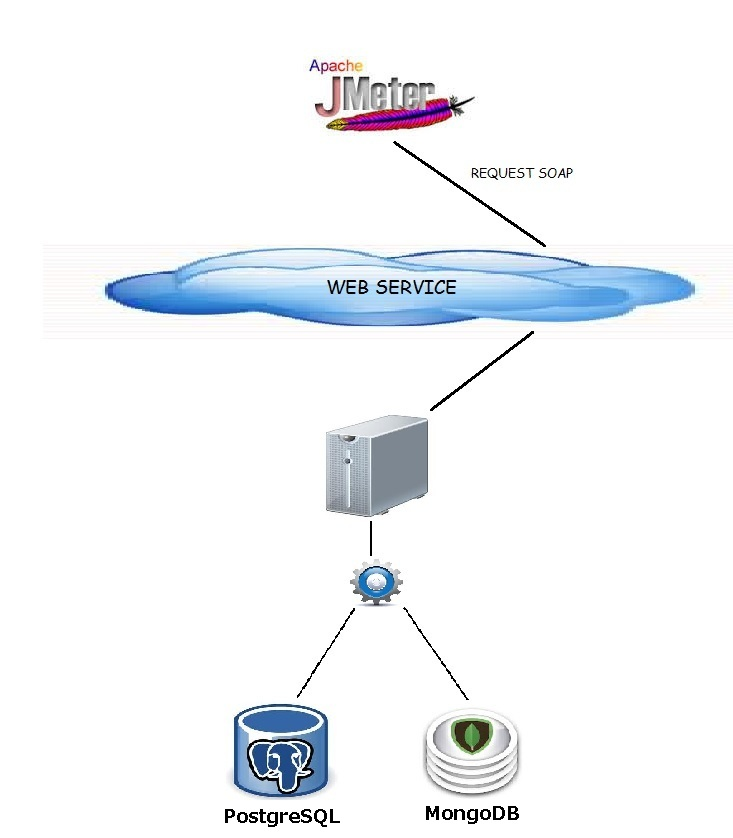
\includegraphics[width=0.5\textwidth]{arquitetura}
		\end{center}
		\caption{Arquitetura de Testes}
		\label{fig:arquitetura}
	\end{figure}

A escolha da linguagem de programação python se deve à facilidade de encontrar os drivers de diversos bancos de dados relacionais e não relacionais, além de ser uma linguagem orientada a objetos e que a utilização vem aumentando. O framework de web2py foi adicionado ao projeto pelo motivo de suportar a implementação de Web services de modo rápido e fácil, altém da geração automática do WSDL (arquivo que contém a descrição das operações do Web service).



\section{web2py}

Web2py é um framework para desenvolvimento ágil de aplicações web, software livre e gratuito. Ele é escrito e programável em Python. [http://www.web2py.com/] web2py foi inspirado pelo Ruby on Rails e Django. Tem seu foco no desenvolvimento ágil e segue o MVC (Model View Controller). Toda aplicação web2py é composta por Models (arquivos que contem a descrição dos dados), Views (arquivos que contem a descrição dos dados que serão apresentados), Controlers (arquivos que contem a lógica e workflow do negócio), Cron Jobs (tarefas que precisam ser executadas regularmente) e Static Files (imagens, scripts, folhas de estilos, etc.)

Quando se trata de Web services, web2py oferece suporte para diversos protocolos, incluindo XML, JSON, RSS,CSV,XMLRPC,JSONRPC,AMFRPC, e SOAP.  O web2py inclui um cliente e servidor SOAP (pysimplesoap) criado por Mariano Reingart. Uma facilidade encontrada é a geração automática do WSDL e a pagina com a descrição dos métodos.


\chapter {Ambiente de Testes}

Os testes foram realizados em uma máquina virtualizada, via VirtualBox, com as seguintes configurações:

\begin{itemize}
\item Sistema Operacional: Debian GNU/Linux 6.0
\item Quantidade de Processadores: 1 
\item Quantidade de Memória RAM: 2048 MB
\item Capacidade do HD: 60 GB
\item Mongo DB: Versão 2.4.0 com configurações padrão
\item PostgreSQL: Versão 8.4.16
\end{itemize}



\chapter{Planos de Teste}

\section{Insere Orgãos}

Esse plano de teste é responsável por medir a performance das inserções de órgãos. Abaixo estão as configurações e os passos do plano de teste.

\subsection{Configurações}

\begin{itemize}
\item Quantidade de usuários virtuais (threads) : 2
\item Tempo de inicialização : 0
\item Quantidade de linhas a serem inseridas: xx
\end{itemize}

\subsection{Sequência de Passos}

\begin{enumerate}
\item Configuração de Dados CSV - É indicado onde está o arquivo csv de onde as threads lerão os valores a serem enviados na requisição soap;
\item Requisição SOAP/XML-RPC - É configurada a URL do Web service e a requisição que será realizada. Cada requisição será montada com os dados lidos do arquivo csv. Cada thread lê uma linha diferente do arquivo.
\item Gráfico de Tempo de Resposta -  Elemento responsável por gerar um gráfico a partir dos dados da requisição feita. O gráfico exibe a  evolução do tempo de resposta das requisições feitas.
\item Gráfico de Resultados - Elemento responsável por exibir a evolução dos tempos das requisições, a média dos tempos das requisições, a derivação do tempo das requisições e a vazão.
\end{enumerate}


\section{Insere Empregados}

Esse plano de teste é responsável por medir a performance das inserções de empregados. Abaixo estão as configurações e os passos do plano de teste.

\subsection{Configurações}

\begin{itemize}
\item Quantidade de usuários virtuais (threads) : 2
\item Tempo de inicialização : 0
\item Quantidade de linhas a serem inseridas: xx
\end{itemize}

\subsection{Sequência de Passos}

\begin{enumerate}
\item Configuração de Dados CSV - É indicado onde está o arquivo csv de onde as threads lerão os valores a serem enviados na requisição soap;
\item Requisição SOAP/XML-RPC - É configurada a URL do Web service e a requisição que será realizada. Cada requisição será montada com os dados lidos do arquivo csv. Cada thread lê uma linha diferente do arquivo.
\item Gráfico de Tempo de Resposta -  Elemento responsável por gerar um gráfico a partir dos dados da requisição feita. O gráfico exibe a  evolução do tempo de resposta das requisições feitas.
\item Gráfico de Resultados - Elemento responsável por exibir a evolução dos tempos das requisições, a média dos tempos das requisições, a derivação do tempo das requisições e a vazão.
\end{enumerate}



